\section{Application details}\label{sec:application}

We implement our nonparametric estimators $\hat{\theta}^{ATE}(d)$, $\hat{\theta}^{\nabla:ATE}(d)$, and $\hat{\theta}^{CATE}(d,v)$ described in Section~\ref{sec:algorithm} (\texttt{RKHS}, solid).  We also implement the nonparametric estimator of \cite{colangelo2020double} (\texttt{DR2}, dashes) using default settings in \texttt{Python} code shared by the authors. Specifically, we use random forest for prediction, with the suggested hyperparameter values. Finally, we implement the semiparametric estimator of \cite{singh2021debiased} (\texttt{DR3}, vertical bars) with 95\% confidence intervals. Specifically, we reduce the continuous treatment into a discrete treatment that takes nine values corresponding to the roughly equiprobable bins $[40,250]$, $(250,500]$, $(500,750]$ $(750,1000]$, $(1000,1250]$, $(1250,1500]$, $(1500,1750]$, and $(1750,2000]$ class hours. Across estimators, we use the tuning procedure described in Supplement~\ref{sec:tuning}. Specifically, we use ridge penalties determined by leave-one-out cross validation, and product exponentiated quadratic kernel with lengthscales set by the median heuristic. 

\begin{figure}[H]
\begin{centering}
     \begin{subfigure}[b]{0.45\textwidth}
         \centering
         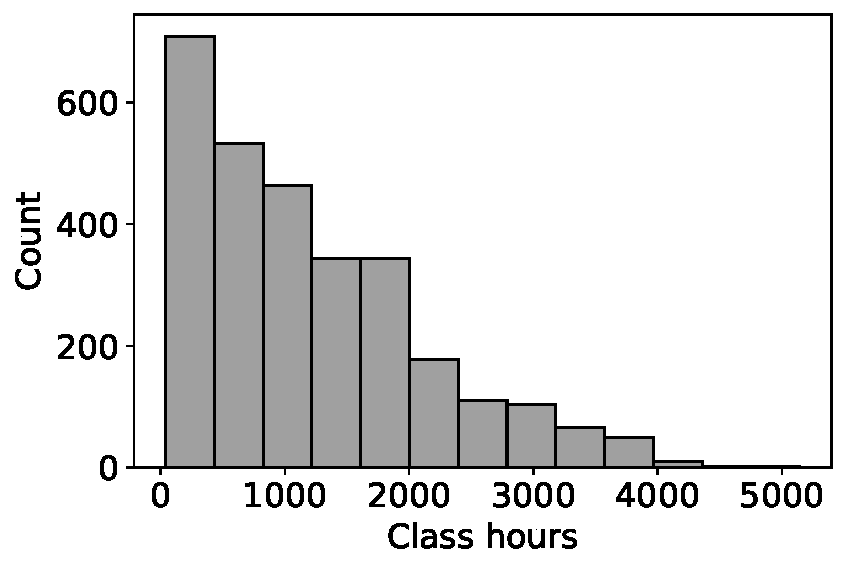
\includegraphics[width=\textwidth]{img/hist_dm_filter_bma.pdf}
         \vspace{-15pt}
         \caption{$D\geq 40$ and $Y>0$.}
     \end{subfigure}
     \hfill
     \begin{subfigure}[b]{0.45\textwidth}
         \centering
         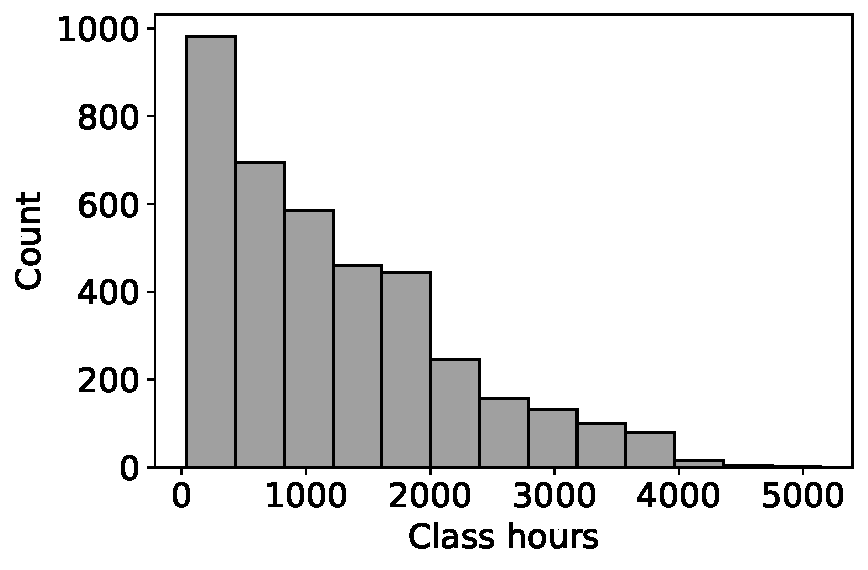
\includegraphics[width=\textwidth]{img/hist_d_filter_bma.pdf}
         \vspace{-15pt}
         \caption{$D\geq 40$.}
     \end{subfigure}
\par
\caption{\label{fig:hist}
Class hours for different samples.}
\end{centering}
\end{figure}


%\vspace{-5pt}
\begin{figure}[ht]
\begin{centering}
     \begin{subfigure}[b]{0.45\textwidth}
         \centering
         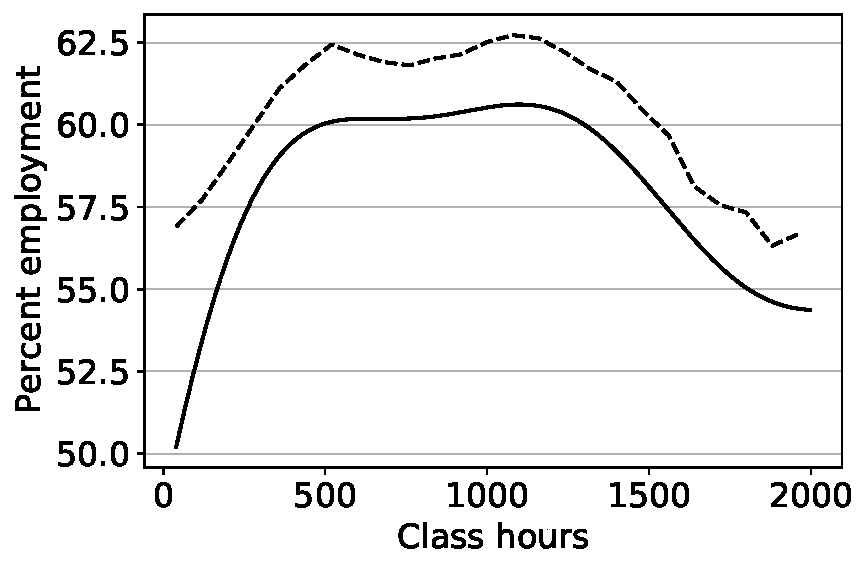
\includegraphics[width=\textwidth]{img/ATE_JCdata_dm_filter_with_dml_bma.pdf}
         %\vspace{-20pt}
         \caption{Dose response curve.}
     \end{subfigure}
     \hfill
     \begin{subfigure}[b]{0.45\textwidth}
         \centering
         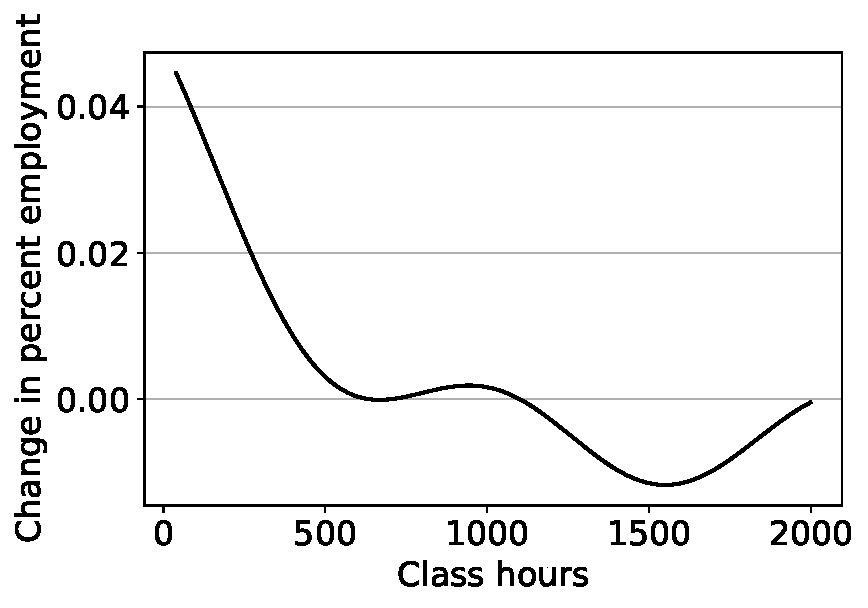
\includegraphics[width=\textwidth]{img/Incremental_ATE_JCdata_dm_filter_bma.pdf}
         %\vspace{-20pt}
         \caption{Incremental response curve.}
     \end{subfigure}
     \vskip\baselineskip
     \begin{subfigure}[b]{0.45\textwidth}
         \centering
         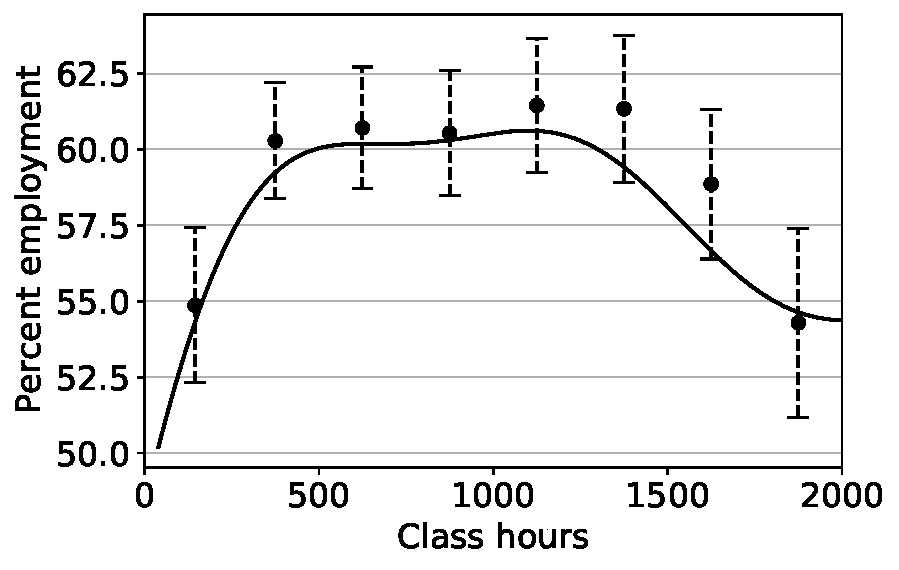
\includegraphics[width=\textwidth]{img/ATE_JCdata_dm_filter_ci_fine_gaussian2_bma.pdf}
         %\vspace{-20pt}
         \caption{Discrete treatment effects.}
     \end{subfigure}
     \hfill
     \begin{subfigure}[b]{0.45\textwidth}
         \centering
         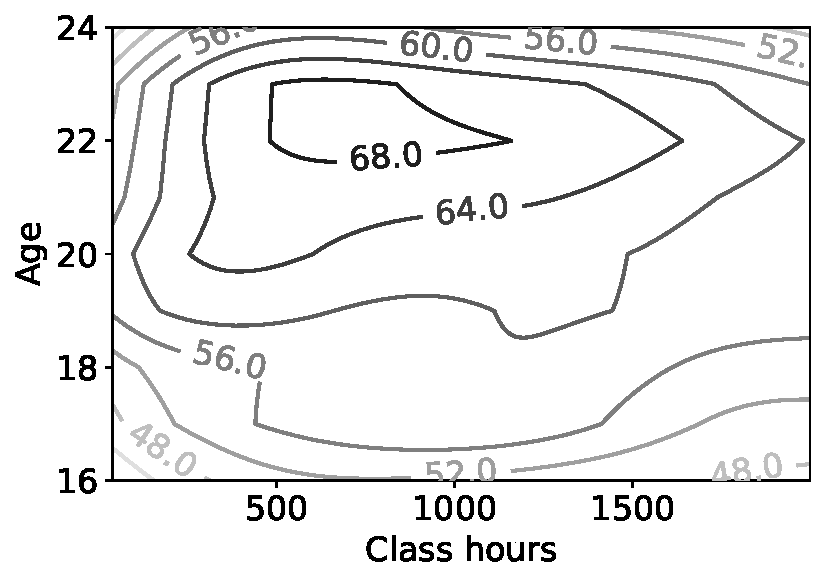
\includegraphics[width=\textwidth]{img/CATE_Age_JCdata_dm_filter_bma.pdf}
         %\vspace{-20pt}
         \caption{Heterogeneous response curve.}
     \end{subfigure}
\par
%\vspace{-10pt}
\caption{\label{fig:JC_d}
Effect of job training on employment: $D\geq 40$ and $Y>0$. We implement our estimators for dose, heterogeneous, and incremental response curves (\texttt{RKHS}, solid). For comparison, we also implement the dose response curve estimator of \cite{colangelo2020double} (\texttt{DR2}, dashes) as well as the discrete treatment effects of \cite{singh2021debiased} (\texttt{DR3}, vertical bars).}
\end{centering}
\end{figure}

We use the dataset published by \cite{huber2020direct}. In Supplement~\ref{sec:experiments}, we focus on the $n=3,906$ observations for which $D\geq 40$, i.e. individuals who completed at least one week of training. In this section, we verify that our results are robust to the choice of sample. Specifically, we consider the sample with $D\geq 40$ and $Y>0$, i.e. the $n=2,989$ individuals who completed at least one week of training and who found employment. 



For each sample, we visualize class hours $D$ with a histogram in Figure~\ref{fig:hist}. The class hour distribution in the sample with $D\geq 40$ and $Y>0$ is similar to the class hour distribution in the sample with $D\geq 40$ that we use in Supplement~\ref{sec:experiments}. Next, we estimate the dose, heterogeneous, and incremental response curve for the new sample choice. Figure~\ref{fig:JC_d} % and~\ref{fig:JC_full} 
visualizes results. For the sample with $D\geq 40$ and $Y>0$, the results mirror the results of the sample with $D\geq 40$ presented in Supplement~\ref{sec:experiments}. Excluding observations for which $Y=0$ leads to estimates that have the same shape but higher magnitudes, confirming the robustness of the results we present in Supplement~\ref{sec:experiments}. 
